\documentclass[border=10pt]{standalone}
\usepackage[T1]{fontenc}
\usepackage{helvet}
\renewcommand{\familydefault}{\sfdefault}
\usepackage{tikz}
\usetikzlibrary{arrows.meta,positioning,calc,decorations.pathreplacing,fit}

\definecolor{idpblue}{HTML}{005DAA}
\definecolor{idpcyan}{HTML}{00B3FF}
\definecolor{warm}{HTML}{D7263D}
\definecolor{inkgray}{HTML}{444444}
\definecolor{forestgreen}{HTML}{2E7D32}

\begin{document}
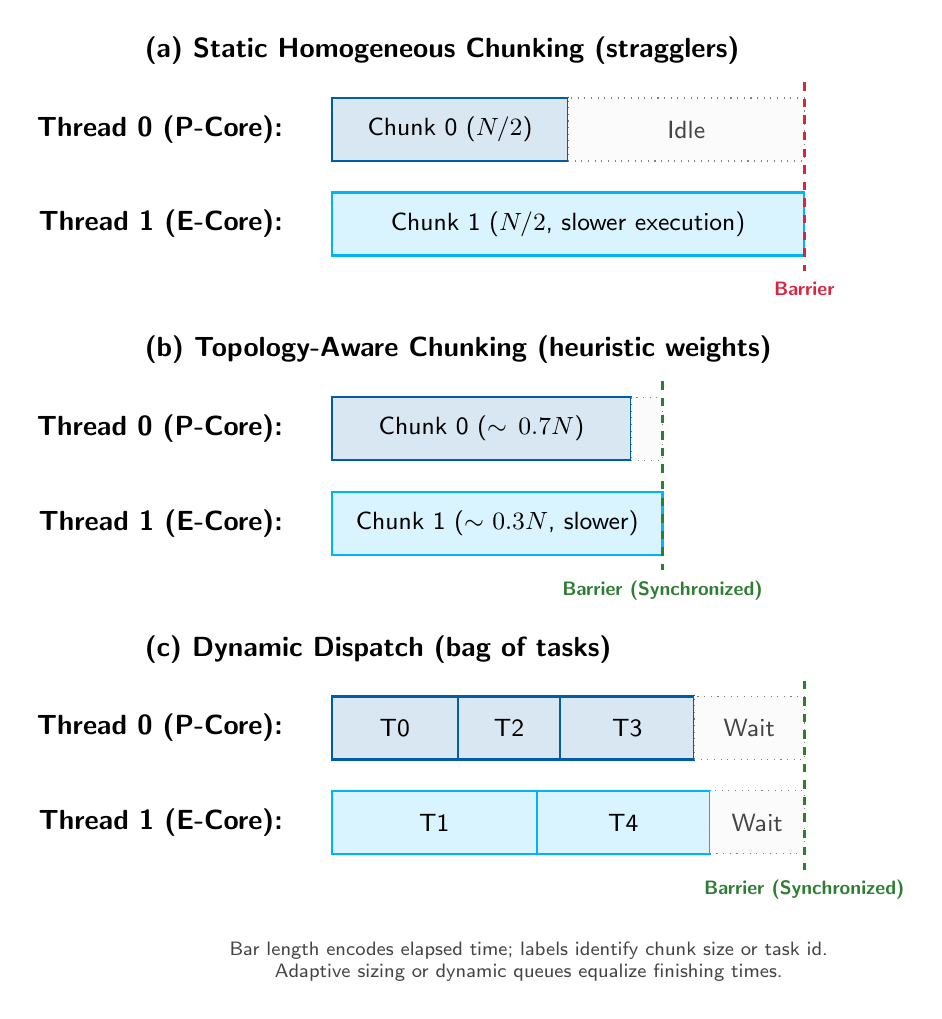
\begin{tikzpicture}[
    font=\small,
    >={Stealth[length=2.2mm]},
    title/.style={font=\bfseries},
    bar/.style={draw=inkgray, minimum height=8mm, align=center, fill=gray!6},
    pcore/.style={bar, fill=idpblue!15, draw=idpblue, thick},
    ecore/.style={bar, fill=idpcyan!15, draw=idpcyan, thick},
    idle/.style={bar, fill=gray!3, draw=gray, dotted, text=inkgray},
    task/.style={draw=inkgray, rounded corners=1pt, fill=idpblue!10, font=\scriptsize\ttfamily},
    label/.style={font=\bfseries},
    barrier/.style={draw=warm, dashed, line width=1.0pt},
]

    % =====================================================================
    % (a) STATIC HOMOGENEOUS CHUNKING
    % =====================================================================
    \node[title, anchor=west] at (-2.5, 4.0) {(a) Static Homogeneous Chunking (stragglers)};
    
    \node[label, anchor=east] at (-0.5, 3.0) {Thread 0 (P-Core):};
    \node[pcore, minimum width=30mm, text width=26mm] (h_t0) at (1.5, 3.0) {Chunk 0 ($N/2$)};
    \node[idle, minimum width=30mm, text width=26mm] (h_t0_wait) at (4.5, 3.0) {Idle};
    
    \node[label, anchor=east] at (-0.5, 1.8) {Thread 1 (E-Core):};
    \node[ecore, minimum width=60mm, text width=56mm] (h_t1) at (3.0, 1.8) {Chunk 1 ($N/2$, slower execution)};
    
    \draw[barrier] (6.0, 3.6) -- (6.0, 1.2) node[below, font=\scriptsize\bfseries\color{warm}] {Barrier};

    % =====================================================================
    % (b) TOPOLOGY-AWARE (FREQUENCY-WEIGHTED)
    % =====================================================================
    \begin{scope}[yshift=-3.8cm]
        \node[title, anchor=west] at (-2.5, 4.0) {(b) Topology-Aware Chunking (heuristic weights)};
        
        \node[label, anchor=east] at (-0.5, 3.0) {Thread 0 (P-Core):};
        \node[pcore, minimum width=38mm, text width=34mm] (w_t0) at (1.9, 3.0) {Chunk 0 ($\sim 0.7N$)};
        \node[idle, minimum width=4mm] (w_t0_wait) at (4.0, 3.0) {};
        
        \node[label, anchor=east] at (-0.5, 1.8) {Thread 1 (E-Core):};
        \node[ecore, minimum width=42mm, text width=38mm] (w_t1) at (2.1, 1.8) {Chunk 1 ($\sim 0.3N$, slower)};
        
        \draw[barrier, draw=forestgreen] (4.2, 3.6) -- (4.2, 1.2) node[below, font=\scriptsize\bfseries\color{forestgreen}] {Barrier (Synchronized)};
    \end{scope}

    % =====================================================================
    % (c) DYNAMIC DISPATCH (BAG OF TASKS)
    % =====================================================================
    \begin{scope}[yshift=-7.6cm]
        \node[title, anchor=west] at (-2.5, 4.0) {(c) Dynamic Dispatch (bag of tasks)};
        
        \node[label, anchor=east] at (-0.5, 3.0) {Thread 0 (P-Core):};
        \node[pcore, minimum width=16mm] (d_t0_1) at (0.8, 3.0) {T0};
        \node[pcore, minimum width=13mm] (d_t0_2) at (2.25, 3.0) {T2};
        \node[pcore, minimum width=17mm] (d_t0_3) at (3.75, 3.0) {T3};
        \node[idle, minimum width=14mm] (d_t0_w) at (5.3, 3.0) {Wait};
        
        \node[label, anchor=east] at (-0.5, 1.8) {Thread 1 (E-Core):};
        \node[ecore, minimum width=26mm] (d_t1_1) at (1.3, 1.8) {T1};
        \node[ecore, minimum width=22mm] (d_t1_2) at (3.7, 1.8) {T4};
        \node[idle, minimum width=12mm] (d_t1_w) at (5.4, 1.8) {Wait};
        
        \draw[barrier, draw=forestgreen] (6.0, 3.6) -- (6.0, 1.2) node[below, font=\scriptsize\bfseries\color{forestgreen}] {Barrier (Synchronized)};
        
        % Legend or source note space
        \node[anchor=north, text=inkgray, font=\scriptsize, align=center] at (2.5, 0.4)
            {Bar length encodes elapsed time; labels identify chunk size or task id.\\
             Adaptive sizing or dynamic queues equalize finishing times.};
    \end{scope}

\end{tikzpicture}
\end{document}
